\documentclass[12pt]{article}

%\usepackage{showframe} %This line can be used to clearly show the new margins
\usepackage{geometry}
\newgeometry{vmargin={25mm, 30mm}, hmargin={15mm,15mm}}   % set the margins

\usepackage{fancyhdr}
\pagestyle{fancyplain}

\usepackage{xcolor}
\usepackage{color}
\definecolor{headercolor}{rgb}{0.3922,0.5843,0.9294}

\usepackage{blindtext}%
\usepackage[theorems,breakable]{tcolorbox}%

\usepackage{tikz} % https://texample.net/tikz/examples/bisector/
\usetikzlibrary{calc,intersections}
\usepackage{tkz-euclide}

\usepackage{amsmath}

\usepackage{enumitem}


\fancypagestyle{cheader}{% https://tex.stackexchange.com/questions/69950/fancyhdr-color-and-width-of-line
	\fancyhf{}% Clear all headers/footers
	\fancyhead[L]{\raisebox{-.5\baselineskip}[0pt][0pt]{Mathematics}}% Header Centred
	\fancyhead[C]{\raisebox{-.5\baselineskip}[0pt][0pt]{\textbf{\Large Center}}}% Header Centred
	\fancyhead[R]{\raisebox{-.5\baselineskip}[0pt][0pt]{\today}}% Header Centred
	\fancyfoot[C]{-\hspace{5mm}\thepage\hspace{5mm}-}% Footer Centred
	\renewcommand{\headrulewidth}{2pt}% 2pt header rule
	\renewcommand{\headrule}{\hbox to\headwidth{%
			\color{headercolor}\leaders\hrule height \headrulewidth\hfill}}
	\renewcommand{\footrulewidth}{0pt}% No footer rule
}

\newtcbtheorem{problem}{Problem}{% https://tex.stackexchange.com/questions/198820/create-newshadetheorem-without-numbering
	theorem name,%
	colback=green!5,%
	colframe=green!35!black,%
	fonttitle=\bfseries,title after break={Problem  -- \raggedleft Continued}%
}{problem}

%\newtcbtheorem{solution}{Solution}{%
%	theorem name,%
%	colback=green!5,%
%	colframe=green!35!black,%
%	fonttitle=\bfseries,title after break={Solution  -- \raggedleft Continued}%
%}{solution}

\linespread{1.2}
\begin{document}
	\pagestyle{cheader}

	\begin{problem}{}{}

		\textit{Given an acute triangle $\triangle ABC$, construct with straightedge and compass square $DEFG$
		such that D and E are on $\overline{BC}$, G is on $\overline{AB}$ and F is on $\overline{AC}$.}
	\end{problem}

	\noindent
	Straightedge and compass can construct the middle point of a line segment, and perpendicular line
	through a point on a line segment.

	\begin{center}
	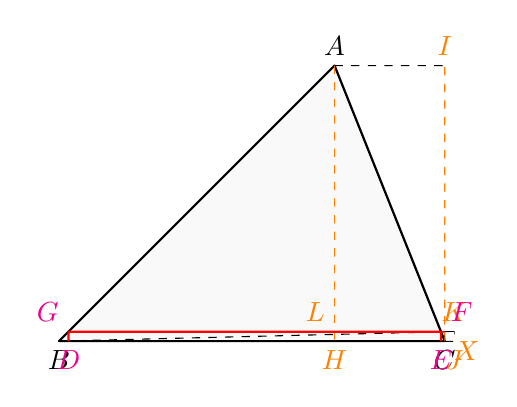
\begin{tikzpicture} [scale=0.7]
		%----------------------------------------------------
		% Coordinates of A, B and C, the triangle vertices
		%----------------------------------------------------
		\tkzDefPoint (5, 5){A}
		\tkzDefPoint (0, 0){B}
		\tkzDefPoint (7, 0){C}
		\tkzLabelPoints[above](A)
		\tkzLabelPoints[below](B,C)
		\tkzDrawPolygon[thick,fill=gray!5](A,B,C);

		\tkzDefPointBy[projection = onto B--C](A) \tkzGetPoint{H};
		\draw [orange, dashed] (A) -- (H) node [right, below] {$H$};

		\tkzDefLine[orthogonal=through C](B,C) \tkzGetPoint{X1};
		\tkzDefLine[parallel=through A](B,C) \tkzGetPoint{X2};
		\tkzInterLL(A,X2)(C,X1) \tkzGetPoint{X3};
		\draw [dashed] (A) -- (X3) node [orange, right, above] {$I$};
		\draw [orange, dashed] (C) -- (X3);

		\tkzCalcLength(C,X3) \tkzGetLength{height};
		\tkzDefShiftPoint[C](\height pt,0){J};
		\draw [dashed] (C) -- (J) node [orange, right, below] {$J$};
		\tkzDefSquare(C,J)\tkzGetPoints{K}{I};
		\tkzDrawPolygon[dashed, color=black](C,J,K, I);
		\draw [dashed] (B) -- (K) node [orange, right, above] {$K$};

		\tkzInterLL(C,I)(B,K) \tkzGetPoint{X};
		\tkzLabelPoint[orange,below right](X){$X$};
		%\tkzAutoLabelPoints(X);
		\tkzDefLine[parallel=through X](B,C) \tkzGetPoint{W};
		\tkzInterLL(X,W)(A,B) \tkzGetPoint{G};
		\tkzInterLL(X,W)(A,C) \tkzGetPoint{F};
		\draw [red, dashed] (F) -- (X);
		\draw [red, thick] (G) -- (F);

		\tkzDefPointBy[projection=onto B--C](F) \tkzGetPoint{E};
		\draw [red, thick] (E) -- (F);
		\tkzDefPointBy[projection=onto B--C](G) \tkzGetPoint{D};
		\draw [red, thick] (G) -- (D);

		\tkzLabelPoint[magenta,below](E){$E$};
		\tkzLabelPoint[magenta,below](D){$D$};
		\tkzLabelPoint[magenta,above right](F){$F$};
		\tkzLabelPoint[magenta,above left](G){$G$};

		\tkzInterLL(F,G)(A,H) \tkzGetPoint{L};
		\tkzLabelPoint[orange,above left](L){$L$};

	\end{tikzpicture}
	\end{center}

	\noindent
	Construction steps are:
	% https://tex.stackexchange.com/questions/119919/no-spacing-between-enumerated-items-with-usepackageenumerate
	\begin{enumerate}[topsep=0pt,itemsep=-1ex,partopsep=1ex,parsep=1ex]
		\item draw height $AH$ to $BC$
		\item extend $BC$ to J such that $CJ$ = $AH$
		\item draw square $CJKI$
		\item set intersection of $CK$ and $BJ$ to $X$
		\item draw line pass $X$ and parallel to $BC$, intersect with $AB$ at $G$, with $AC$ at $F$
		\item draw perpendicular lines down from $G$ and $F$ to get $D$ and $E$
	\end{enumerate}

	\noindent
	To prove $DEFG$ is a square, since $\triangle BCX \sim \triangle BJK$,
	\begin{equation}
		\frac{CX}{JK} = \frac{BC}{BJ}
		\quad \textrm{or} \quad \frac{EF}{AH} = \frac{BC}{BC + AH}
		\quad \textrm{or} \quad EF = \frac{BC * AH}{BC + AH}
	\end{equation}
	since $\triangle ABC \sim \triangle AGF$,
	\begin{equation}
		\frac{GF}{BC} = \frac{AL}{AH} = \frac{AH - EF}{AH}
	\end{equation}
	Then we just need to verify that $GF = EF$. From $(2)$,
	\begin{equation}
		\begin{aligned}
		GF &= BC * \frac{AH - EF}{AH} = \frac{BC}{AH} *(AH - EF)\\
		   &= \frac{BC}{AH} * (AH - \frac{BC * AH}{BC + AH}), \quad from (1)\\
		   &= \frac{BC}{AH} * \frac{AH^2}{BC + AH} = \frac{BC * AH}{BC + AH} = EF
		\end{aligned}
	\end{equation}

	\noindent
	The construction logic is derived from the $GF$ expression.

	This\\
	is \\
	a \\
	long \\
	solution\\
	spilled\\
	to\\
	page\\
	2
\end{document}
